\section{Results}
\label{sec:results}

\subsection{H1: entropy is lower, not higher, for hallucinated answers}
\label{sec:h1}

\begin{table}[t]
    \centering
    \caption{\Hone: relative difference in mean final-three-layer attention entropy, hallucinated versus factual, with 95\% bootstrap CIs. Negative values mean lower entropy for hallucinated answers. No estimate comes near the hypothesized $+15\%$ to $+30\%$ band, and the large pooled difference mostly disappears within domains.}
    \label{tab:h1}
    \resizebox{\textwidth}{!}{%
    \begin{tabular}{@{}lcc@{}}
        \toprule
        \textbf{Scope} & \qwen & \llama \\
        \midrule
        Pooled (confounded by domain) & $-18.4\%$ \ci{$-19.4$}{$-17.3$}, $d=-0.70$ & $-14.7\%$ \ci{$-15.4$}{$-14.0$}, $d=-0.91$ \\
        \midrule
        biography & $-0.8\%$ \ci{$-3.5$}{$+1.8$} & $-3.7\%$ \ci{$-5.0$}{$-2.4$} \\
        geography & $+2.1\%$ \ci{$-0.7$}{$+4.9$} & $-4.5\%$ \ci{$-5.9$}{$-3.0$} \\
        creative works & $-6.0\%$ \ci{$-11.5$}{$-0.6$} & $-14.1\%$ \ci{$-16.3$}{$-11.9$} \\
        science & $-2.9\%$ \ci{$-5.4$}{$-0.4$} & $-4.5\%$ \ci{$-5.6$}{$-3.4$} \\
        trivia & $-9.1\%$ \ci{$-11.7$}{$-6.7$} & $-9.8\%$ \ci{$-11.5$}{$-8.0$} \\
        \midrule
        OLS, domain fixed effects + length & $-2.1\%$ \ci{$-3.2$}{$-0.9$} & $-6.4\%$ \ci{$-7.1$}{$-5.7$} \\
        \bottomrule
    \end{tabular}
    }
\end{table}


\begin{figure}[t]
    \centering
    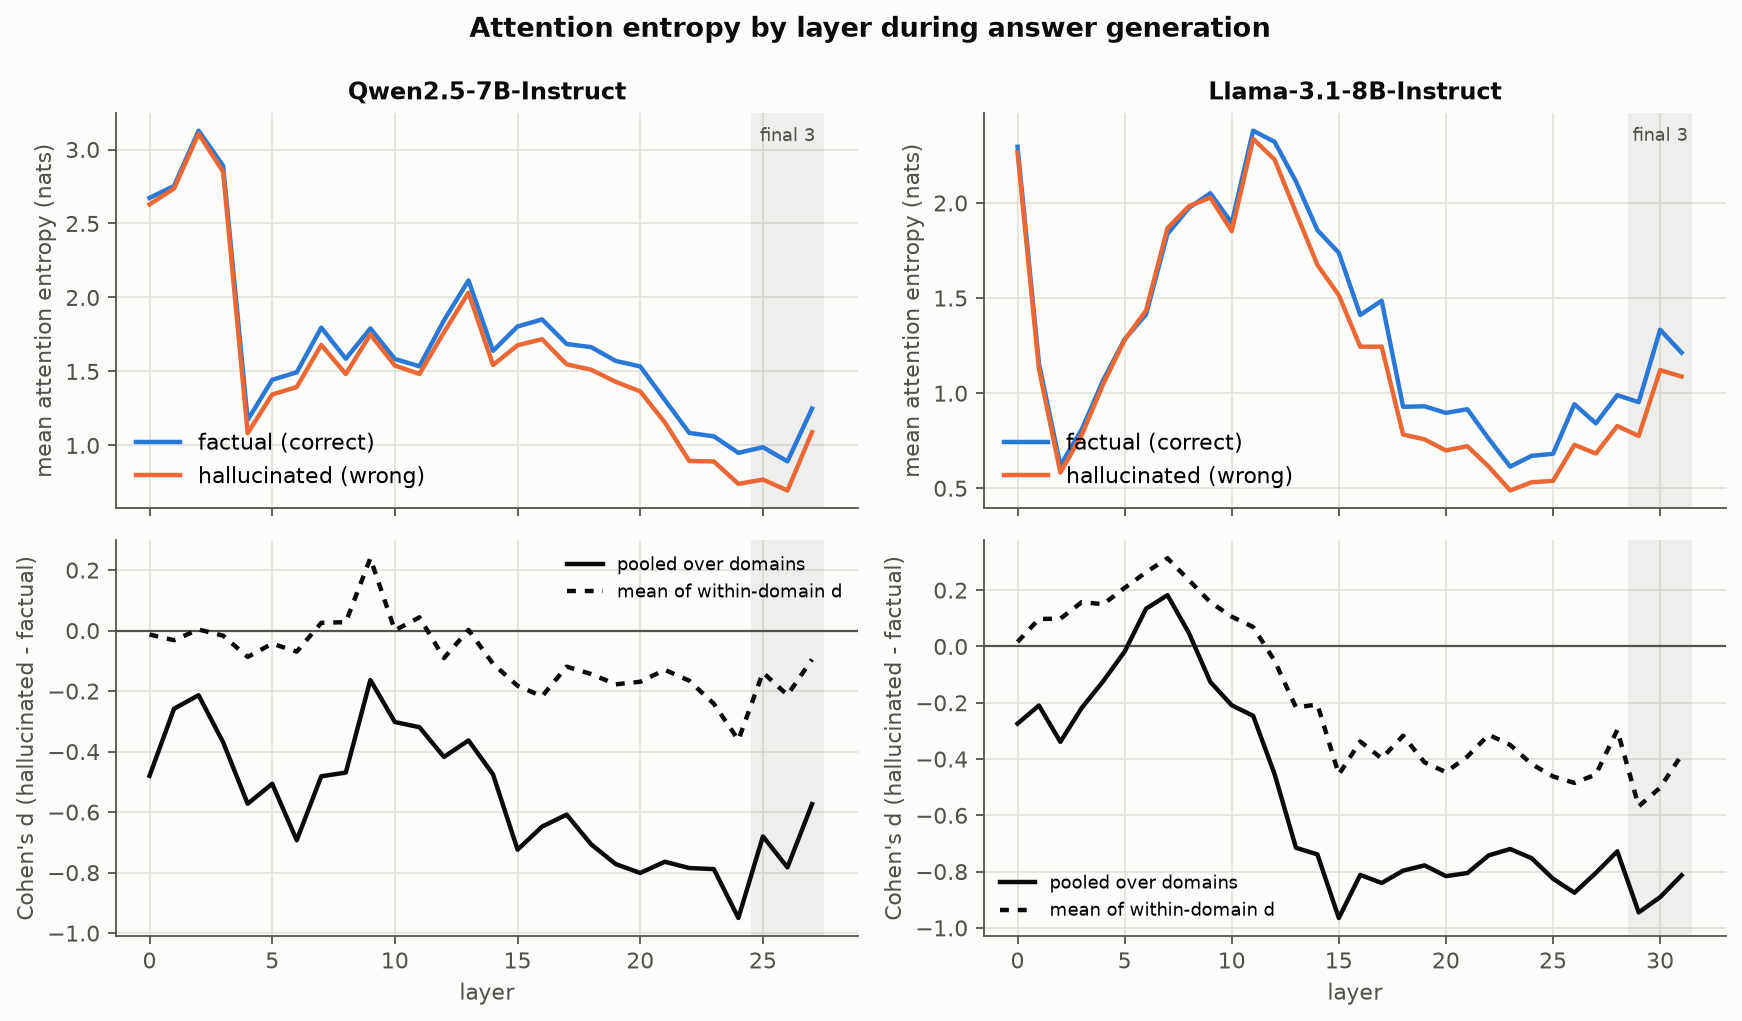
\includegraphics[width=0.95\linewidth]{figures/fig1_layer_profile.png}
    \caption{Attention entropy by layer during answer generation. \textbf{Top:} mean entropy for factual and hallucinated answers, pooled over domains; the shaded band marks the final three layers. \textbf{Bottom:} Cohen's $d$ (hallucinated minus factual), pooled (solid) and averaged over within-domain estimates (dashed). Hallucinated answers have lower entropy in the upper half of both networks. Within domains, the difference is near zero or slightly positive in early-to-middle layers and much smaller than the pooled curve suggests.}
    \label{fig:layer_profile}
\end{figure}

\Tabref{tab:h1} reports the relative difference in final-three-layer entropy.
Pooled over domains, hallucinated answers have 18.4\% lower entropy in \qwen (0.851 versus 1.043 nats) and 14.7\% lower in \llama (0.995 versus 1.166 nats).
No estimate in either model, pooled or within a domain, comes near the hypothesized $+15\%$ to $+30\%$ band.
We reject \Hone: the sign is reversed.

{\bf How much of the pooled difference is real?}
Most of it is a between-domain artifact.
The \popqa domains have both shorter prompts with lower entropy and far more wrong answers, so pooling mixes a domain difference into the hallucination difference.
Within domains, the difference ranges from $-14.1\%$ to $+2.1\%$, and two of the ten within-domain intervals include zero (\figref{fig:last3}).
With domain fixed effects and length covariates, the adjusted difference is $-2.1\%$ \ci{$-3.2$}{$-0.9$} for \qwen and $-6.4\%$ \ci{$-7.1$}{$-5.7$} for \llama.
The effect is therefore real but small, and it is clearer in \llama than in \qwen.

\begin{figure}[t]
    \centering
    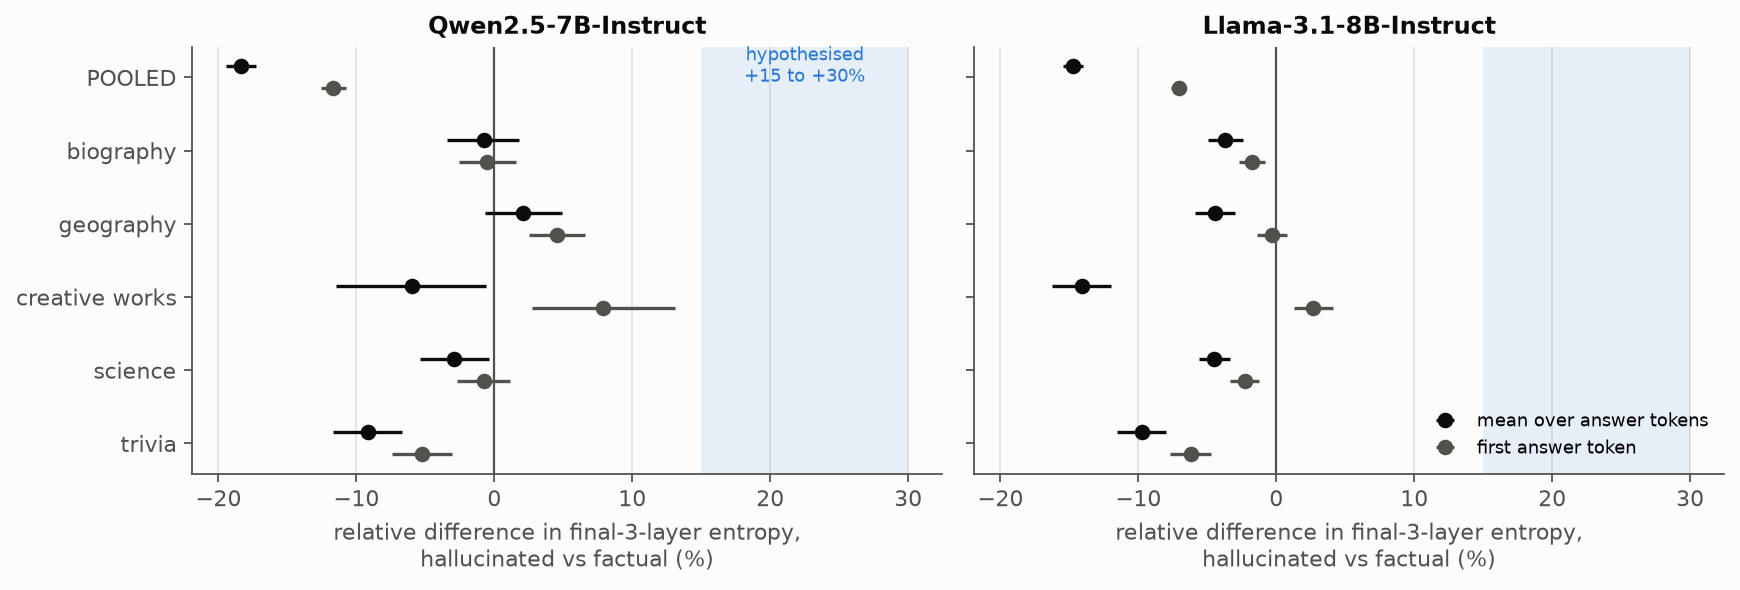
\includegraphics[width=0.95\linewidth]{figures/fig2_last3_effect.png}
    \caption{Relative difference in final-three-layer entropy, hallucinated versus factual, with 95\% CIs, for the answer-mean feature (black) and the first-answer-token feature (gray). The shaded band is the hypothesized $+15\%$ to $+30\%$ range. Every estimate falls outside it, and the first-token feature does not even have a consistent sign across domains.}
    \label{fig:last3}
\end{figure}

\para{Robustness.}
The result does not depend on our analysis choices.
Length normalization changes nothing material: the pooled difference is $-17.6\%$ and $-14.1\%$.
Label choice does not matter either: the pooled difference is $-17.9\%$ and $-14.2\%$ with judge-only labels and $-15.3\%$ and $-12.7\%$ with string-match labels.
The first-token feature is the one variant that behaves differently.
Its within-domain difference ranges from $-6.2\%$ to $+7.9\%$, with a domain average of $+1.2\%$ for \qwen and $-1.6\%$ for \llama, so at the moment the model starts its answer there is no consistent entropy shift in the final three layers.

\para{Layer profile.}
\Figref{fig:layer_profile} shows why a single late-layer average is a poor summary.
Entropy differences are near zero or slightly positive in early-to-middle layers and negative in the upper half of the network.
In \llama, the within-domain effect peaks at $d \approx +0.3$ around layer 7 and falls to between $-0.3$ and $-0.5$ in the upper layers.
Pooled, the difference is significant after FDR correction in 28 of 28 layers for \qwen and 30 of 32 for \llama, but this pooled significance inherits the domain confound.

\subsection{H2: pooled AUROC clears 0.75, but mostly for the wrong reason}
\label{sec:h2}

\begin{table}[t]
    \centering
    \caption{\Htwo: classifiers trained on all domains pooled. \emph{Pooled} is the AUROC of out-of-fold scores with a 95\% bootstrap CI; \emph{Within} is the mean over the five domains of the AUROC of the same scores computed inside each domain. A domain indicator alone reaches 0.785 / 0.723 pooled, so pooled numbers overstate every detector. Best result per column in \textbf{bold}.}
    \label{tab:h2}
    \resizebox{\textwidth}{!}{%
    \begin{tabular}{@{}lcccc@{}}
        \toprule
        & \multicolumn{2}{c}{\qwen} & \multicolumn{2}{c}{\llama} \\
        \cmidrule(lr){2-3} \cmidrule(lr){4-5}
        \textbf{Features} & Pooled & Within & Pooled & Within \\
        \midrule
        \multicolumn{5}{@{}l}{\emph{Controls}} \\
        domain indicator only & 0.785 \ci{0.774}{0.796} & 0.429 & 0.723 \ci{0.711}{0.736} & 0.423 \\
        length only & 0.669 \ci{0.657}{0.681} & 0.527 & 0.652 \ci{0.639}{0.664} & 0.535 \\
        \midrule
        \multicolumn{5}{@{}l}{\emph{Attention entropy}} \\
        final-3-layer mean (1 feature) & 0.700 \ci{0.688}{0.711} & 0.539 & 0.731 \ci{0.720}{0.742} & 0.638 \\
        layer-wise, answer mean (primary) & 0.827 \ci{0.817}{0.836} & 0.719 & 0.817 \ci{0.807}{0.826} & 0.740 \\
        layer-wise, first answer token & 0.826 \ci{0.816}{0.835} & 0.683 & 0.821 \ci{0.812}{0.830} & 0.743 \\
        layer-wise, length-normalized & 0.826 \ci{0.817}{0.835} & 0.718 & 0.815 \ci{0.806}{0.825} & 0.740 \\
        layer-wise + length & 0.833 \ci{0.824}{0.842} & 0.727 & 0.822 \ci{0.813}{0.831} & 0.747 \\
        per-head ($L \times H$ features) & 0.890 \ci{0.883}{0.898} & 0.821 & 0.874 \ci{0.867}{0.882} & 0.830 \\
        \midrule
        \multicolumn{5}{@{}l}{\emph{Token likelihood}} \\
        logit baseline & 0.876 \ci{0.868}{0.884} & 0.812 & 0.878 \ci{0.870}{0.886} & 0.847 \\
        layer-wise entropy + logit & {\bf 0.891} \ci{0.884}{0.899} & {\bf 0.823} & {\bf 0.890} \ci{0.883}{0.898} & {\bf 0.854} \\
        \bottomrule
    \end{tabular}
    }
\end{table}


\begin{figure}[t]
    \centering
    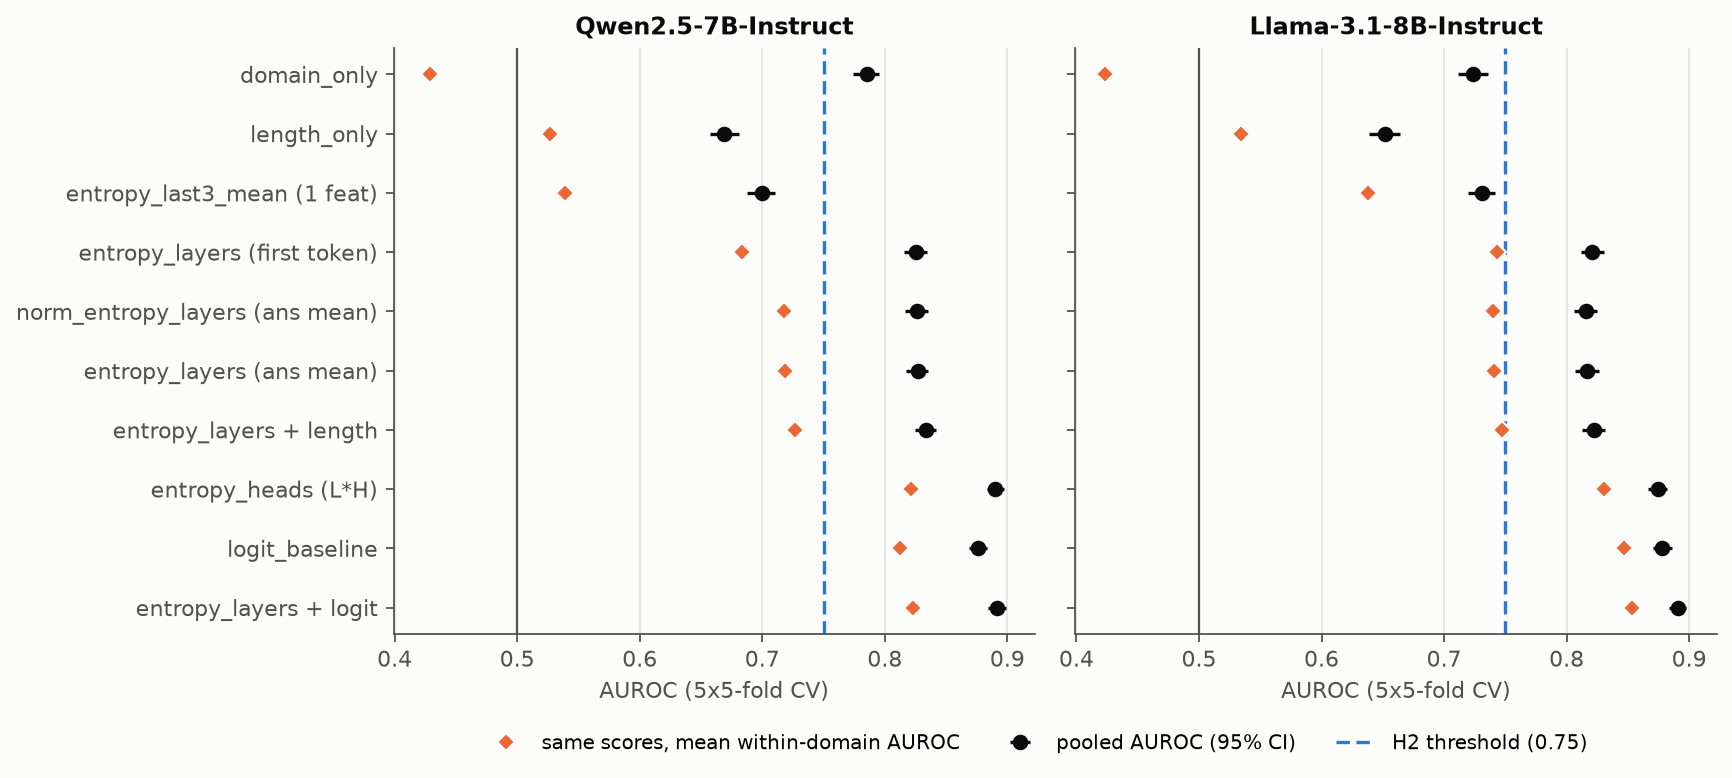
\includegraphics[width=0.95\linewidth]{figures/fig3_auroc_feature_sets.png}
    \caption{AUROC by feature set for classifiers trained on pooled data. Black points are pooled AUROC with 95\% CIs; orange diamonds are the mean within-domain AUROC of the same scores; the dashed line is the \Htwo threshold of 0.75. Every pooled number sits well above its within-domain counterpart, and the domain indicator alone clears or approaches the threshold.}
    \label{fig:auroc_sets}
\end{figure}

By the pre-specified criterion, \Htwo passes in both models: layer-wise entropy reaches a pooled AUROC of 0.827 \ci{0.817}{0.836} for \qwen and 0.817 \ci{0.807}{0.826} for \llama (\tabref{tab:h2}).
The result is stable: the standard deviation of AUROC across the five cross-validation repeats is below 0.001.

{\bf Does this number mean what it appears to mean?}
Not quite.
A classifier that sees only which of the five domains a question comes from already reaches 0.785 and 0.723, because hallucination rates range from 23\% to 94\% across domains (\tabref{tab:data}) and layer-wise entropy encodes domain.
Layer-wise entropy beats this domain-only control by $+0.041$ \ci{0.032}{0.051} for \qwen and $+0.093$ \ci{0.082}{0.105} for \llama.
When we score the same out-of-fold predictions inside each domain, the mean AUROC drops to 0.719 and 0.740 (\figref{fig:auroc_sets}).
We therefore read \Htwo as mixed: the criterion is met, but most of the margin over chance could be obtained from the domain alone.

\para{The hypothesized feature is weak.}
The specific statistic in \Hone and \Htwo, the mean entropy of the final three layers, reaches only 0.700 and 0.731 pooled and 0.539 and 0.638 within domain.
The full layer profile is needed to get a usable detector.

\para{Entropy is not a length artifact.}
Layer-wise entropy beats the length-only control by $+0.158$ \ci{0.145}{0.170} and $+0.165$ \ci{0.152}{0.178} AUROC.
Normalizing entropy by $\log n_p$ or adding length features changes pooled AUROC by less than 0.01.

\para{Token likelihood is a stronger signal.}
The logit baseline reaches 0.876 and 0.878, which is 0.049 \ci{0.040}{0.058} and 0.062 \ci{0.053}{0.070} above layer-wise entropy.
Adding entropy to the logit baseline gains $+0.015$ \ci{0.010}{0.020} and $+0.012$ \ci{0.009}{0.016}.
The gain is statistically reliable but small.

\para{Averaging over heads loses signal.}
Per-head entropy reaches 0.890 and 0.874 pooled and 0.821 and 0.830 within domain, about 0.10 above per-layer entropy within domain and comparable to the logit baseline.
Most of the usable attention signal lives in individual heads and is lost when we average a layer.

\subsection{H3: science is hardest, but biography is not easiest}
\label{sec:h3}

\begin{table}[t]
    \centering
    \caption{\Hthree: AUROC of classifiers trained and cross-validated inside each domain. The entropy rows carry 95\% bootstrap CIs. Science is the lowest domain for layer-wise entropy in both models; biography is third. Best domain per row in \textbf{bold}.}
    \label{tab:h3}
    \resizebox{\textwidth}{!}{%
    \begin{tabular}{@{}llcccccc@{}}
        \toprule
        & \textbf{Features} & biography & geography & creative works & science & trivia & mean \\
        \midrule
        \multirow{4}{*}{\qwen}
        & layer-wise entropy & 0.747 \ci{0.716}{0.775} & 0.802 \ci{0.777}{0.824} & {\bf 0.892} \ci{0.857}{0.922} & 0.616 \ci{0.581}{0.648} & 0.711 \ci{0.684}{0.736} & 0.753 \\
        & length only & 0.507 & 0.599 & 0.552 & 0.546 & 0.593 & 0.559 \\
        & logit baseline & 0.781 & 0.800 & {\bf 0.911} & 0.728 & 0.853 & 0.815 \\
        & entropy + logit & 0.810 & 0.860 & {\bf 0.932} & 0.730 & 0.839 & 0.834 \\
        \midrule
        \multirow{4}{*}{\llama}
        & layer-wise entropy & 0.742 \ci{0.713}{0.768} & {\bf 0.831} \ci{0.808}{0.851} & 0.820 \ci{0.792}{0.846} & 0.694 \ci{0.664}{0.722} & 0.741 \ci{0.711}{0.769} & 0.765 \\
        & length only & 0.423 & {\bf 0.655} & 0.633 & 0.584 & 0.491 & 0.557 \\
        & logit baseline & 0.827 & 0.853 & {\bf 0.885} & 0.792 & 0.879 & 0.847 \\
        & entropy + logit & 0.845 & 0.877 & {\bf 0.896} & 0.813 & 0.883 & 0.863 \\
        \bottomrule
    \end{tabular}
    }
\end{table}


\begin{figure}[t]
    \centering
    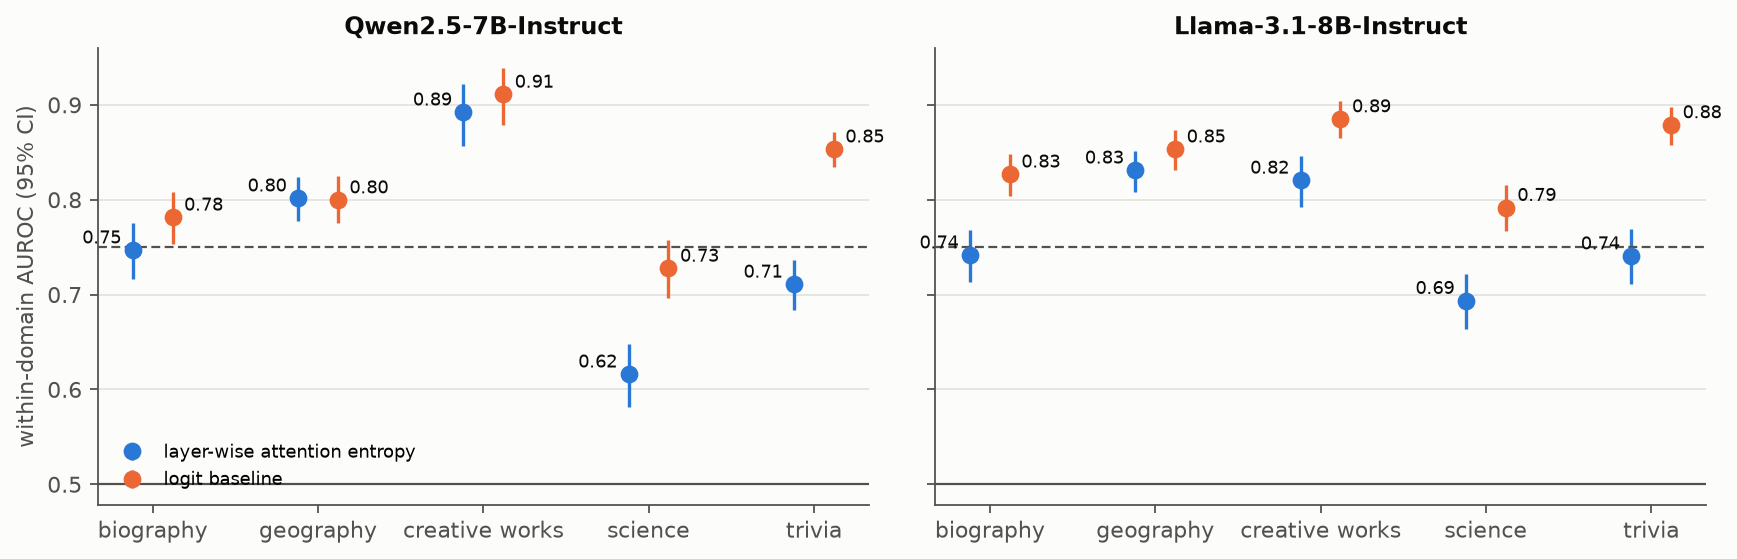
\includegraphics[width=0.95\linewidth]{figures/fig4_auroc_by_domain.png}
    \caption{Within-domain AUROC with 95\% CIs for layer-wise attention entropy (blue) and the logit baseline (orange). The dashed line marks 0.75. Science is the lowest domain for entropy in both models, and the logit baseline dips there too. Entropy trails the logit baseline most on trivia.}
    \label{fig:auroc_domain}
\end{figure}

\Tabref{tab:h3} reports classifiers trained and cross-validated inside each domain.
Layer-wise entropy averages 0.753 for \qwen and 0.765 for \llama, with a range of 0.616 to 0.892.
Only geography and creative works exceed 0.75 in both models.

\para{Science is lowest.}
Science has the lowest AUROC in both models, 0.616 and 0.694.
The bootstrap probability that science is the lowest domain is 1.00 for \qwen and 0.98 for \llama, and the ordering holds under all three labelings.
The logit baseline shows the same dip (0.728 and 0.792), so the weakness in science is not specific to attention features (\figref{fig:auroc_domain}).

Combining entropy with the logit baseline raises the within-domain mean from 0.815 to 0.834 for \qwen and from 0.847 to 0.863 for \llama, but the gain is not uniform: on trivia for \qwen the combination (0.839) is below the logit baseline alone (0.853).

\para{Biography is not highest.}
Biography ranks third of five in both models under the primary labels, behind creative works and geography, and it is never the top domain in any bootstrap resample.
In \llama, biography and trivia are effectively tied (0.742 versus 0.741), and biography falls to fourth under both alternative labelings.
Biography does beat science, by $+0.131$ \ci{0.083}{0.176} in \qwen and $+0.048$ \ci{0.009}{0.088} in \llama.
\Hthree is thus half supported.

\para{Cross-domain transfer.}
Training on one domain and testing on another gives a mean off-diagonal AUROC of 0.651 for \qwen and 0.682 for \llama, against 0.753 and 0.765 within domain (\figref{fig:transfer}).
Part of the signal generalizes across domains and part is domain-specific.
Transfer is uneven: in \qwen, classifiers trained on any other domain reach 0.73 to 0.88 on creative works, while no classifier trained elsewhere exceeds 0.60 on science.

\begin{figure}[t]
    \centering
    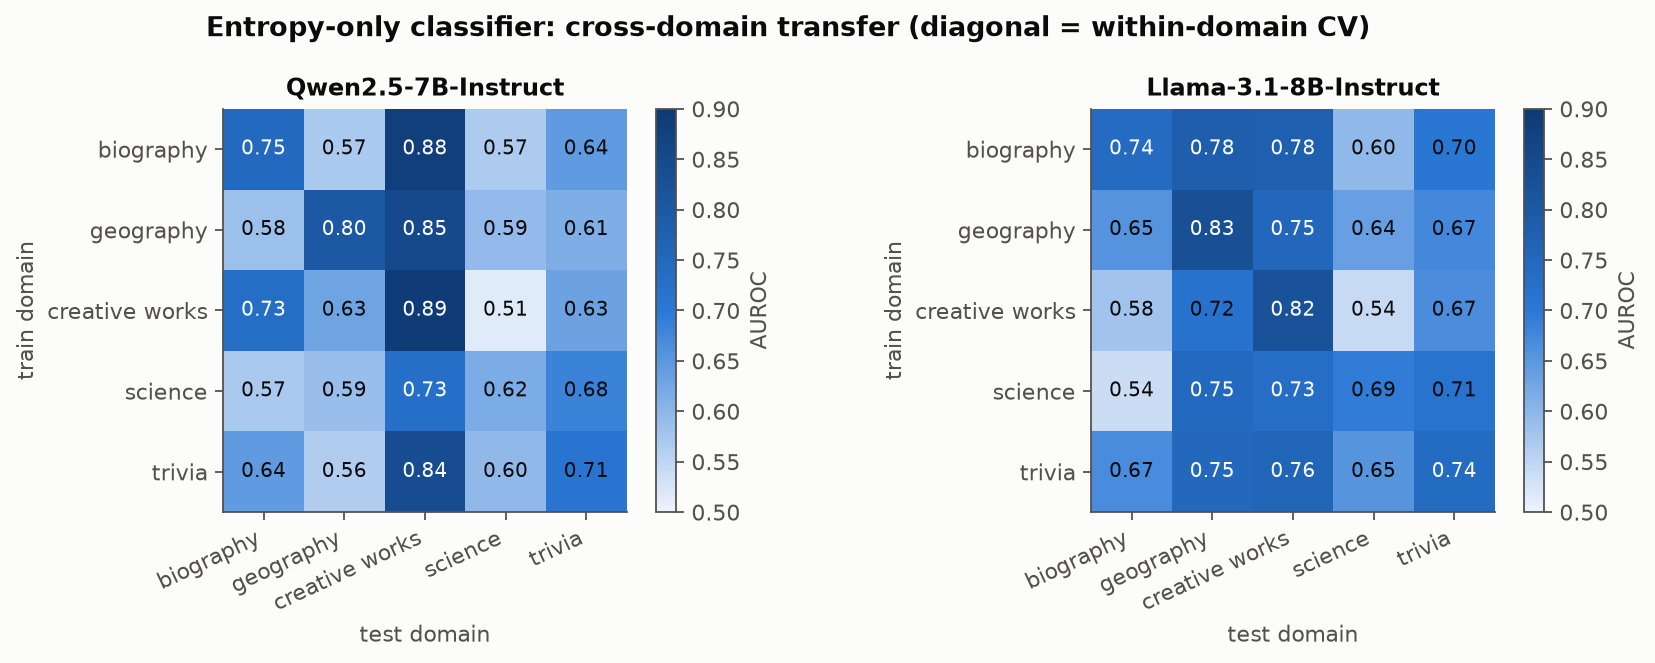
\includegraphics[width=0.9\linewidth]{figures/fig5_transfer.png}
    \caption{Cross-domain transfer of the layer-wise entropy classifier. Rows are training domains and columns are test domains; the diagonal is within-domain cross-validated AUROC. Off-diagonal cells average 0.651 (\qwen) and 0.682 (\llama), so the signal transfers only partly. Science is the hardest test domain to transfer into in both models.}
    \label{fig:transfer}
\end{figure}

\subsection{Error analysis}
\label{sec:errors}

\para{By relation.}
Within \popqa, the pooled entropy classifier is strongest on \emph{capital} (0.85 for \qwen, 0.84 for \llama) and, for \qwen, on \emph{author} and \emph{screenwriter} (0.88 to 0.91).
For \qwen it is weakest on \emph{father}, \emph{place of birth}, \emph{country}, and \emph{capital of} (0.66 to 0.68).
\Tabref{tab:relation} in the appendix lists all relations.

\para{Missed hallucinations.}
Misses cluster in science and trivia questions where the model gives a fluent, confident near-miss, such as ``Bone marrow'' for the skeleton, or ``pharaoh'' for the Sphinx's human head.
These answers often have very low token negative log-likelihood as well, so token likelihood does not flag them either.

\para{False alarms.}
False alarms are mostly correct answers about obscure \popqa entities, such as the screenwriter of \emph{A Special Day}, where the question looks like the ones the model usually gets wrong.

\para{Label noise.}
Some apparent misses are label errors: ``Belgium'' for the origin of French fries is graded wrong against the gold answer.

\para{Overlap with token likelihood.}
Entropy and logit scores are correlated but not redundant, with a within-domain Spearman correlation of 0.33 for \qwen and 0.50 for \llama.
This is consistent with the small gain from combining them.
